% $Id: SpacecraftDesign.tex,v 1.2 2008/10/09 16:16:11 dconway Exp $
\chapter{\label{chapter:Spacecraft}SpaceObjects: Spacecraft and Formation Classes}
\chapauthor{Darrel J. Conway}{Thinking Systems, Inc.}

The Spacecraft and Formation classes used in GMAT are the core components studied when running the
system. Instances of these classes serve to model spacecraft state information as the model
evolves.  They also serve as containers for hardware components used to extend the model to include
finite burn analysis, contact calculations, spatial mass distributions, and full six degree of
freedom modeling.  The core elements of this modeling are presented in this chapter.  The hardware
extensions are documented in Chapter~\ref{chapter:Hardware}.

\section{Component Overview}

The central nature of Spacecraft and Formation objects in GMAT's mission model makes the design of
the supported features of these classes potentially quite complex.  The state data and related
object properties required for these objects must meet numerous requirements, including all of the
following:

\begin{enumerate}
\item Supply State information to force model
\begin{itemize}
\item Origin dependent data, MJ2000 Earth Equator orientation
\item Cartesian states
\item  <<Future>> Equinoctial states
\end{itemize}
\item  Support input representations
\begin{itemize}
\item  Convert between different representations
\item  Preserve accuracy of input data
\end{itemize}
\item Support coordinate systems
\begin{itemize}
\item  Support internal MJ2000 Cartesian system for propagation
\item  Allow state inputs in different systems
\item  Show state in different systems on demand
\end{itemize}
\item  Support time systems
\begin{itemize}
\item TAI ModJulian based internal time system
\item Support ModJulian
\item Support Gregorian
\item Convert all time systems
\end{itemize}
\item  Support mass and ballistic properties
\begin{itemize}
\item Basic spacecraft mass
\item Cd, Cr, Areas
\item Mass in tanks
\item <<Future>> Mass depletion from maneuvers
\item <<Future>> Moments of Inertia
\end{itemize}
\item  Support tanks and thrusters
\begin{itemize}
\item Add and remove tanks and thrusters
\item <<Future>> Deplete mass during finite burn
\item <<Future, partially implemented>> Model burn direction based on thruster orientations (BCS
based)
\end{itemize}
\item GUI
\begin{itemize}
\item Provide epoch information
\begin{itemize}
\item Epoch representation string
\item Epoch in that representation
\item Supply different representation on request
\item Preserve precision of input epoch data
\end{itemize}
\item Provide state information
\begin{itemize}
\item State type string
\item State in that representation
\item Provide units and labels for state elements
\item Convert to different representations
\item Preserve precision of input state data
\end{itemize}
\item Provide support for finite maneuvers
\end{itemize}
\item Scripting
\begin{itemize}
\item Support all GUI functionality from scripting
\item Provide element by element manipulations of state data
\item Allow element entry for data not in the current state type without forcing a state type change
\end{itemize}
\item Provide Range Checking and Validation for all Editable Data
\item <<Future>> Support attitude
\begin{itemize}
\item Allow attitude input
\item Convert attitude states
\end{itemize}
\item  <<Future>> Support sensors
\begin{itemize}
\item Add and remove
\item Conical modeling
\item Masking
\item Contact information based on sensor pointing (BCS based)
\end{itemize}
\end{enumerate}


GMAT defines a base class, SpaceObject, for the common elements shared by spacecraft and
formations.  The primary feature of the SpaceObject class is that it provides the data structures
and processes necessary for propagation using GMAT's numerical integrators and force models.
Classes are derived from this base to capture the unique characteristics of spacecraft and
formations.  Additional components that interface with the propagation subsystem should be added to
GMAT in this hierarchy; the propagation subsystem is designed to work at the SpaceObject level.

The SpaceObject subsystem uses three categories of helper classes: PropStates, Converters, and
Hardware.  In one sense, the SpaceObject classes can be viewed as containers supporting the
features needed to model objects in the solar system that evolve over time through numerical
integration in GMAT.

The core data needed for propagation is contained in the PropState helper class.  Each SpaceObject
has one PropState instance used to manage the data directly manipulated by the numerical
integrators.  The PropState manages the core epoch and state data used by the propagation subsystem
to model the SpaceObjects as they evolve through time.  Details of the PropState class are given in
Section~\ref{section:PropState}.

Each SpaceObject includes components used to take the data in the PropState and convert it into a
format appropriate for viewing and user interaction. The conversion subsystem described in
Section~\ref{section:ConversionClasses} provides the utilities needed to convert epoch data,
coordinate systems, and state element representations.  The conversion routines needed to meet the
requirements are contained in a triad of conversion classes: TimeConverter, CoordinateConverter, and
RepresentationConverter, that share a common base that enforces consistent interfaces into the
conversion routines.  These conversion routines interact with the state and epoch data at the
SpaceObject level on GMAT; therefore, conversions on a Formation object are performed using
identical calls to conversions for individual Spacecraft.  In other words, the state or epoch data
for a Formation is transformed for all members of the Formation with a single call, and that call
looks identical to the same transformation when performed on a single spacecraft.

The spacecraft as modeled in GMAT is a fairly simple object, consisting of several key properties
required to model ballistics and solar radiation forces.  The state complexities are managed in the
SpaceObject base class.  Additional spacecraft hardware -- fuel tanks, thrusters, and eventually
sensors and other hardware elements -- are modeled as configurable hardware elements that are added
as needed to Spacecraft objects.  Hardware elements that contribute to the spacecraft model are
broken out into separate classes modeling the specific attributes of those elements. Users configure
fuel tanks and thrusters as entities that the spacecraft uses for finite maneuvering.  These
elements include structures that allow location and orientation configuration in the Spacecraft's
body coordinate system, so that detailed mass and moment data can be calculated during the mission.
A future release of GMAT will add support for attitude calculations and, eventually, sensors, so
that attitude based maneuvering, full six degree of freedom modeling, and detailed contact modeling
can be incorporated into the system.   These components are discussed in more detail in
Chapter~\ref{chapter:Hardware}.

The remainder of this chapter details the design of the components that implement the core
SpaceObject classes, Spacecraft and Formation.  It includes the design specification for the
converters GMAT uses to support these classes, along with a discussion of how these elements
interact to provide the conversions needed to meet the system requirements.

\section{Classes Used for Spacecraft and Formations}

Figure~\ref{figure:SpacecraftandFormation} shows the details of the classes derived from SpacePoint
that are used when modeling spacecraft and formations of spacecraft.  The class hierarchy
for the spacecraft subsystem consists of three core classes: the SpaceObject class, which contains
the common elements of the subsystem, the Spacecraft class, which acts as the core component for all
spacecraft modeling, and the Formation class, which collects spacecraft and subformations into a
single unit for modeling purposes.  This subsystem also contains a helper class, the PropState,
which encapsulates the data that evolves as the model is run, simplifying the interface to the
propagation subsystem.  In addition, two of the hardware classes -- Thruster and FuelTank -- are
shown in the figure.

\begin{figure}
\begin{center}
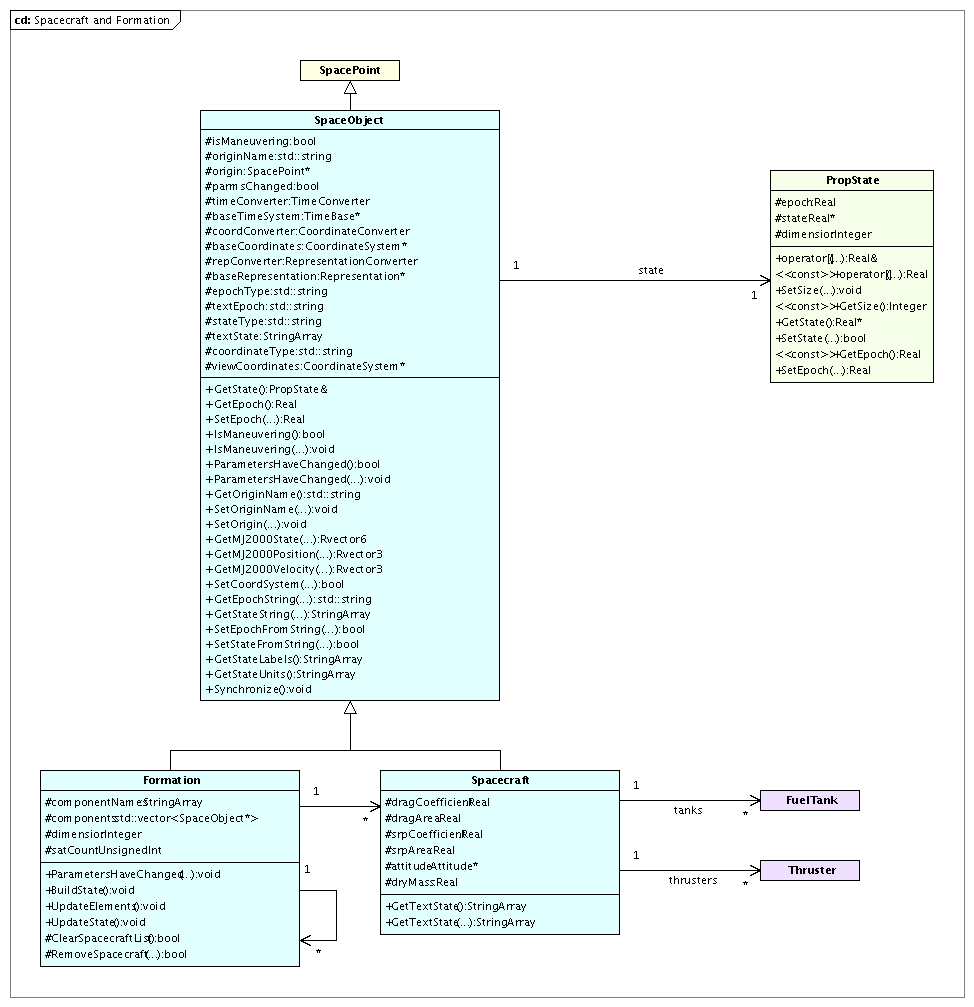
\includegraphics[scale=0.45]{Images/SpacecraftandFormation.eps}
\caption{\label{figure:SpacecraftandFormation}Class Structure for Spacecraft and Formations}
\end{center}
\end{figure}

\subsection{Design Considerations}

The central role of the Spacecraft and Formation SpaceObjects in GMAT's models drives several
design considerations related to the consistent display and use of these objects in the model.
Before presenting the design of the classes used for these objects, several of the considerations
that went into this design will be discussed.

\subsubsection{Data Consistency Philosophy}

The SpaceObject subsystem follows a convention that requires that the state data in the PropState
always stays correct with respect to the model.  In other words, once some data in the state vector
is set, changes to other properties of the SpaceObject do not change the state with respect to the
model.  That means that if the internal origin changes for a SpaceObject, the data in the state
vector is translated to the new location, and the velocity data is updated to reflect the speed of
the SpaceObject with respect to the new origin.  In order to change the state of a SpaceObject in
GMAT's model, the actual state data must be changed.  Changing the coordinate system or origin does
not change the position or velocity of the SpaceObject with respect to other objects in the space
environment; instead, it changes the values viewed for the SpaceObject by updating the viewed data
in the new coordinate system.  The epoch also remains unchanged upon change of the coordinate
system, the representation, or elements of the state vector.

Epoch data is simpler (because it is independent of location in the space environment), but follows
the same philosophy.  Internally the epoch data is stored in the TAI modified Julian time system.
Users can view the epoch data in any of GMAT's defined time systems.  Changing the time system does
not change the internal epoch data, only the way that data is presented.  Epoch data is changes by
directly updating the epoch.  Upon change of epoch, the state of the spacecraft remains unchanged
with respect to the SpaceObject's origin.  However, a side effect of changing the epoch on a
SpaceObject is that the locations of the objects in the solar system may shift, so the location of
the SpaceObject with respect to other solar system objects may be different.

\subsubsection{Data Presented to the User}

Each SpaceObject includes data members used to track the current default views of the data.  The
epochType member is used to store the current format for viewing the epoch data.  State data
requires two components to fully define the view of the state data: the coordinateType member tracks
the coordinate system used to view the state data, and the stateType member the representation for
that view of the state data.  These three members -- epochType, coordinateType, and stateType --
define the views used when a SpaceObject is written to a file, displayed on a GUI panel, or accessed
as strings for other purposes.

Access to the state and epoch data as Real values returns the internal data elements: the epoch
is returned as a TAI modified Julian value, and the state data is returned as Cartesian
Mean-of-J2000 Earth equatorial data, referenced to the origin specified for the SpaceObject.  The
SpaceObjects provide methods that retrieve the data in other formats as well; the values described
here are those returned using the default GetRealParameter methods overridden from the GmatBase
class.

State data can be read or written either element by element or as a vector of state data.  The
former approach is taken by the Script Interpreter when setting a spacecraft's state as expressed
element-by-element in the script, like shown here:

\begin{quote}
\begin{verbatim}
Create Spacecraft sat;
sat.StateType = Keplerian;
sat.SMA = 42165.0;
sat.ECC = 0.0011;
sat.INC = 0.25;
sat.RAAN = 312.0;
sat.AOP = 90.0;
sat.TA = 270.0;
\end{verbatim}
\end{quote}

\noindent The GUI works with the state data as a single entity, rather than element-by-element.
Accordingly, the panel that displays spacecraft state data accesses this data with a single call
that returns the full state data\footnote{A future release of GMAT will provide a scripting option
to set the full state in a single script line, using the format

\begin{quote}
\texttt{Create Spacecraft sat;\\
sat.StateType = Keplerian;\\
sat.State = [42165.0, 0.0011, 0.25, 312.0, 90.0, 270.0];}
\end{quote}}.

Spacecraft states can be displayed in many different representations.  Rather than code text
descriptions for the different components of each representation into the representation converter,
each representation includes structures to provide the labels and units used for the components.
The SpaceObjects provide methods to retrieve these values.

Some state representations have optional settings for specific elements.  For example, the Keplerian
representation can specify the anomaly in one of several forms: elliptical states can specify a true
anomaly, eccentric anomaly, or mean anomaly, while hyperbolic orbits use either the hyperbolic
anomaly or a mean anomaly defined off of the hyperbolic anomaly.  Representations that support this
type of option also provide a method, SetOption(), to set the option.  SpaceObjects provide methods
to access these methods as well, so that the representation options can be set through calls to the
SpaceObject.

\subsection{The SpaceObject Class}

GMAT's force model constructs a state vector that is manipulated by the system's numerical
integrators to advance the state vector through time, as described in
Chapter~\ref{chapter:Propagators}.  The core building block for the construction of this state
vector is the SpaceObject, a class used in GMAT as the base class for Spacecraft and
Formations\footnote{A future release will include the State Transition Matrix (STM) in the
SpaceObject class hierarchy.}, as shown in the class diagram,
Figure~\ref{figure:SpacecraftandFormation}.

The SpaceObject class supports all operations and data elements that Spacecraft and Formations share
in common.  In particular, the vector used by the propagators to model evolution over time is
encapsulated in the SpaceObject class.  Conversions that involve the data in this vector are
performed at the SpaceObject level.  The SpaceObject class maintains pointers to the elements that
are necessary for these conversions.

SpaceObject instances also act as containers for several helper classes, responsible for performing
coordinate system conversions, state transformations between different state representations, and
time system conversions that allow the object's epoch information to be presented to users in common
time systems, described in Section~\ref{section:ConversionClasses}. The SpaceObject class implements
several methods that call those components to supply requested data.  The returned data from these
calls is always an std::string or StringArray.  The SpaceObject class manages the underlying Real
data internally, and uses these as checkpoints to manage the precision of the output, to validate
that the data is consistent, and to ensure that all data presented to the users is consistent with
the internal data structures in the SpaceObject.

\subparagraph{\textit{Class Attributes}}

\begin{itemize}
\item \textbf{PropState state}: The container for the raw state and epoch data that gets
propagated.  Details of the PropState class are provided in Section~\ref{section:PropState}.
\item \textbf{bool isManeuvering}: A flag used to indicate if there is a finite burn active for any
of the members of the SpaceObject.
\item \textbf{std::string originName}: The name of the SpacePoint that is the origin of the data
contained in the SpaceObject's PropState.
\item \textbf{SpacePoint *origin}: A pointer to the SpacePoint that is the origin of the data in
the state.
\item \textbf{bool parmsChanged}: A flag used to indicate if the size or data contained in the
PropState has changed, so that consumers of those data can perform updates.
\item \textbf{SpacePoint *origin}: The origin used for the state data.
\item \textbf{CoordinateSystem *baseCoordinates}: The coordinate system used for the state data.
This coordinate system is a Mean-of-J2000 Earth-Equator system, with the origin set to the
SpaceObject's origin.
\item \textbf{std::string epochType}:  Text descriptor for the current epoch type used for display.
\item \textbf{TimeConverter timeConverter}:  The time converter used by this SpaceObject.
\item \textbf{<<Future>> TimeBase* baseTimeSystem}: The time system matching the epochType.
\item \textbf{std::string coordinateType}: Text descriptor for the current coordinate system used
for display.
\item \textbf{CoordinateConverter coordConverter}:  The coordinate system converter used by this
SpaceObject.
\item \textbf{CoordinateSystem* baseCoordinates}: The coordinate system associated with the
SpaceObject's PropState.
\item \textbf{CoordinateSystem* viewCoordinates}: The coordinate system associated with the
SpaceObject's coordinateType, used for display.
\item \textbf{std::string stateType}: Text descriptor for the current state representation used for
display.
\item \textbf{RepresentationConverter repConverter}:  The representation converter used by this
SpaceObject.
\item \textbf{<<Future>> Representation* baseRepresentation}:  The representation used for display.
\item \textbf{std::string textEpoch}: The most recently accessed string version of the epoch.  This
string is only updated if the epoch field is accessed as a string using GetEpochString(), and the
epoch or epoch type has changed since the last access.
\item \textbf{StringArray textState}: The most recently accessed string version of the state.  This
string array is only updated if the state is accessed as a string array using GetStateString(), and
the coordinate type or representation has changed since the last access.
\end{itemize}

\subparagraph{\textit{Methods}}

\begin{itemize}
\item \textbf{PropState \&GetState()}:  Returns the internal PropState.
\item \textbf{Real GetEpoch()}: Returns the TAI modified Julian epoch of the SpaceObject, obtained
from the PropState.
\item \textbf{Real SetEpoch(Real ep)}: Sets the SpaceObject's epoch to a new value.  The input
parameter is the new TAI epoch.  This mathod passes the new epoch into the PropState for storage.
\item \textbf{bool IsManeuvering()}:  Returns a flag indicating if a finite burn is currently active
for the SpaceObject.
\item \textbf{void IsManeuvering(bool mnvrFlag)}:  Sets the flag indicating the presence of a finite
burn.
\item \textbf{bool ParametersHaveChanged()}:  Returns a flag indicating that the state data has been
changed outside of the propagation subsystem, and therefore the states need to be refreshed.
\item \textbf{void ParametersHaveChanged(bool flag)}:  Method used to indicate that an external
change was made, and therefore states should be refreshed before propagating.
\item \textbf{std::string GetOriginName()}:  Returns the name of the SpacePoint used as the origin
of the state data.
\item \textbf{void SetOriginName(const std::string \&cbName)}:  Sets the name of the origin used for
the state data.
\item \textbf{void SetOrigin(SpacePoint *cb)}:  Sets the SpacePoint corresponding to the origin of
the state vector.  The SpacePoint passed in the parameter cb is the new origin, and gets set on the
base coordinate system as its origin.
\item \textbf{Rvector6 GetMJ2000State(A1Mjd \&atTime)}:  Returns the Cartesian state relative to the
SpaceObject's J2000 body\footnote{The current GetMJ2000 methods take an a.1 epoch as the epoch for
the calculation.  A future release will change this call to use TAI epochs.}.
\item \textbf{Rvector3 GetMJ2000Position(A1Mjd \&atTime)}:  Returns the Cartesian position relative
to the SpaceObject's J2000 body.
\item \textbf{Rvector3 GetMJ2000Velocity(A1Mjd \&atTime)}:  Returns the Cartesian velocity relative
to the SpaceObject's J2000 body.
\item \textbf{bool SetCoordSystem(CoordinateSystem* coordsys)}:  Sets the viewCoordinates member to
the input coordinate system.
\item \textbf{std::string GetEpochString(std::string toTimeType)}:  Returns the current epoch in
string form, in the format in the toTimeType input.  If toTimeType is an empty string, epochType is
used as the format for the output.
\item \textbf{StringArray GetStateString(std::string toType, std::string toCoords, CoordinateSystem*
toCS)}:  Returns the SpaceObject state in the representation specified by toType, in the coordinate
system set by toCoords, using the internal coordinate converter and the input coordinate system,
toCS.  If toCS is NULL, the coordinate converter locates the required coordinate system.  If, in
addition, toCoords is an empty string, viewCoordinates is used for the output coordinate system.  If
the toType is also an empty string, the baseRepresentation is used.
\item \textbf{bool SetEpochFromString(std::string epochString, std::string timeType)}:  Sets the
epoch in the PropState using the input epochString, which is formatted using the input timeType.
\item \textbf{bool SetStateFromString(StringArray stateString, std::string fromType, std::string
fromCoords, CoordinateSystem* fromCS)}:  Sets the state in the PropState using the data in the
stateString array, which has the representation specified in the fromType string in coordinate
system fromCoords, which has an instance in the fromCS input.
\item \textbf{StringArray GetStateLabels()}:  Returns a string array containing the labels
identifying the state elements.
\item \textbf{StringArray GetStateUnits()}:  Returns a string array containing the units for the
state elements.
\item \textbf{void Synchronize()}:  Method used to fill the textEpoch and textState from the data in
the PropState.
\end{itemize}

\subsection{\label{section:PropState}The PropState Class}

All SpaceObjects contain a member PropState element that is designed to encapsulate all data needed
to propagate the SpaceObject.  This member class is used to provide the single state vector
propagated as the core component seen by GMAT's propagators.  The PropState objects can contain data
for a single spacecraft, multiple spacecraft (typically flown in a Formation), and related mass
depletion and state transition matrix data.  The propagator subsystem ensures that these data are
treated appropriately during propagation.

Each PropState instance defined the following data members and methods:

\subparagraph{\textit{Class Attributes}}

\begin{itemize}
\item \textbf{Real epoch}: The current epoch for the state. This value is a TAI modified Julian
value, and is used in the force model to specify the epoch for force evaluations.
\item \textbf{Real* state}: The state vector that gets propagated.
\item \textbf{Integer dimension}: The total number of elements in the state vector.
\end{itemize}

\subparagraph{\textit{Methods}}

\begin{itemize}
\item \textbf{Real \&operator[](const Integer el)}:  Provides element by element access to the state
vector, so that the components can be set using the same syntax as is used to set C++ array
elements.
\item \textbf{Real operator[](const Integer el) const}:  Provides element by element access to the
state vector, so that the components can be read using the same syntax as is used to read C++ array
elements.
\item \textbf{void SetSize(const Integer size)}: Resizes the state vector.  This method copies the
current state data into the resized vector once the new vector has been allocated.
\item \textbf{const Integer GetSize() const}: Returns the current size of the state vector.
\item \textbf{Real *GetState()}: Returns the state vector.  The returned vector is the internal
Cartesian state used by the propagators.  The state data is in Mean-of-J2000 Earth-Equatorial
coordinates, referenced to the SpaceObject's origin.
\item \textbf{bool SetState(Real *data, Integer size)}:  Sets the state vector to match the input
vector. If the size parameter is less than or equal to the dimension of the state vector, the data
vector is copied into the state vector, filling from the start until the indicated number of
elements is filled.  If size is greater than the PropState dimension, the method returns false.  The
input state is in Mean-of-J2000 Earth-Equatorial coordinates, referenced to the SpaceObject's
origin.
\item \textbf{Real GetEpoch() const}: Returns the value of the epoch data member.  The returned
value is a TAI modified Julian value.
\item \textbf{Real SetEpoch(const Real ep)}: Sets the value of the epoch data member.  The input
value is a TAI modified Julian value.
\end{itemize}

\section{The Spacecraft Class}

One key component that supplies PropState data to GMAT is the Spacecraft class, used to model
satellites in the mission control sequence.  Each satellite studied in the mission has a
corresponding Spacecraft object, configured to simulate the behavior of that satellite.  The
Spacecraft contains core data elements necessary to model the physical characteristics of the
satellite, along with the inherited SpaceObject properties that form the core state representations
used for propagation.

In GMAT, the Spacecraft model allows for the addition of new satellite components that model
specific hardware elements.  The current implementation supports fuel tanks and thrusters for use
when modeling finite maneuvers.  The base class for the hardware subsystem was designed to be
flexible, incorporating data elements designed to model the location and orientation of the hardware
relative to a satellite body coordinate system.  The orientation data is used in GMAT to set the
thruster direction during finite burns.  Once the thrust direction has been determined, it it
rotated based on the satellite's attitude to determine the thrust direction in the propagation
frame, so that the maneuver acceleration can be incorporated into the force model.  This modular
hardware incorporation is also the first step towards incorporating moments of inertia into the
model, so that full six degree of freedom modeling can be performed in GMAT.  Additional details of
the hardware model are provided in Chapter~\ref{chapter:Hardware}.

\subsection{Internal Spacecraft Members}

Spacecraft objects are SpaceObjects, so they contain all of the data structures associated with
SpaceObjects described above.  They manage a StringArray that contains the current state as
expressed in the current state representation.  This array typically contains the state as seen on
the GUI or in the script file that configured the Spacecraft; the data in this array is only updated
when needed for display purposes.

The Spacecraft class contains data members controlling the core ballistics of the object.  Mass is
handled as a core Spacecraft mass plus all masses associated with the hardware attached to the
Spacecraft.  The force model accumulates the mass into a total mass used in the acceleration
calculations.  Areas and force coefficients are included in the Spacecraft model for drag and solar
radiation pressure calculations.

\subsection{Spacecraft Members}

The Spacecraft class provides data memebers used to manage the ballistic properties of the
spacecraft.  Properties are defined to manage the spacecraft mass, incident areas for drag and
solar radiation pressure perturbations, associated coefficients of drag and reflectivity, and the
structures needed to add hardware elements to the core spacecraft objects.  The members that
provide this support are:

\subparagraph{\textit{Class Attributes}}

\begin{itemize}
\item \textbf{Real dragCoefficient}: The coefficient of drag, $C_d$ (see equation~\ref{eq:Drag}),
used when calculating atmospheric forces acting on the spacecraft.
\item \textbf{Real dragArea}:  The area of the spacecraft encountering the atmosphere.
\item \textbf{Real srpCoefficient}: The reflectivity coefficient, $C_R$ (see equation~\ref{eq:SRP}),
used when calculating accelerations from solar radiation pressure.
\item \textbf{Real srpArea}: The area exposed to solar radiation, for the purposes of calculating
the solar radiation pressure force.
\item \textbf{Real dryMass}: The total mass of the spacecraft, excluding fuel and other massive
hardware elements.
\item \textbf{StringArray tankNames}: Names of the fuel tanks that the spacecraft uses.
\item \textbf{StringArray thrusterNames}:  Names of the thrusters that the spacecraft uses.
\item \textbf{ObjectArray tanks}:  Array of fuel tanks on the spacecraft.  Fuel tanks are added to
spacecraft by making local copies of defined tanks.  Each fuel tank contributes fuel mass to the
total mass of a spacecraft.  Fuel is depleted from the tanks during finite maneuvers\footnote{Mass
depletion is scheduled for implementation during the summer of 2007.}.
\item \textbf{ObjectArray thrusters}:  Array of thrusters attached to the spacecraft.  Thrusters
are added to spacecraft by making local copies of defined thrusters.  Each thruster has a location
and pointing direction defined in teh spacecraft's body coordinate system.  The applied thrust dir
ection is computed by rotating the thrust direction based on teh spacecraft's
attitude\footnote{The current implementation uses either an inertial attitude or a
velocity-normal-binormal attitude for this calculation.}. The thruster mass should be included in
the dry mass of the spacecraft.
\item \textbf{Real totalMass}: The total mass of the spacecraft, including fuel and other massive
hardware elements.  This is a calculated parameter, available only as an output.  Users cannot set
the spacecraft's total mass.
\end{itemize}

\subparagraph{\textit{Methods}}

The support for Spacecraft state and epoch access and manipulation is provided by the SpaceObject
base class.  Access to the new data members described above is provided using the GmatBase access
methods described in Section~\ref{section:GmatBase}.  Generally speaking, the ballistic properties
are accessed using the GetRealParameter and SetRealParameter methods overrifdden from the base
class.  Hardware elements are set by name, and configured on the Spacecraft by passing in pointers
to configured hardware elements which are then cloned inside the spacecraft tto make the local copy
used when executing the mission control sequence.  Since most of the infrastructure for these steps
is described elsewhere, the list of new methods on the Spacecraft is rather sparse, consisting of
notes describing Spacecraft specific details implemented for these core methods:

\begin{itemize}
\item \textbf{virtual Real GetRealParameter(const Integer id) const}: Returns the real
parameters listed in the data member section.  Of particular interest here is the treatment of the
mass parameter.  Requests can be made for either the dry mass of the spacecraft or the total mass
of the spacecraft.  When the total mass is requested, the returned value is the output of the
UpdateTotalMass() method described below.
\item \textbf{virtual bool TakeAction(const std::string \&action, const std::string
\&actionData~=~"")}: TakeAction in the Spacecraft class adds the following new actions to the
object:
\begin{itemize}
\item \textit{SetupHardware}: Examines the hardware on the spacecraft, and sets up internal
linkages required for this hardware.  For example, each thruster reqires a pointer to a fuel tank;
that connection is configured by this action.
\item \textit{RemoveHardware}: Removes one or all hardware elements from the Spacecraft.  If a name
is specified for the hardware element, only that element is removed.  If the actionData string is
empty, all hardware elements are removed.
\item \textit{RemoveTank}: Removes one or all fuel tanks from the Spacecraft.  If a name is
specified for the fuel tank, only that tank is removed.  If the actionData string is empty, all fuel
tanks are removed.
\item \textit{RemoveThruster}: Removes one or all thrusters from the Spacecraft.  If a name is
specified for the thruster, only that thruster is removed.  If the actionData string is empty, all
thrusters are removed.
\end{itemize}
\end{itemize}

The Spacecraft Class includes the following protected methods used to maintain some of the internal
data structures, and to generate data needed for the public methods:

\begin{itemize}
\item \textbf{Real UpdateTotalMass()}: Updates the total mass by adding all hardware masses to the
dry mass.
\item \textbf{Real UpdateTotalMass() const}: Updates the total mass by adding all hardware masses to
the dry mass.  The const version does not update the internal member, and therefore can be called
by other const methods.
\end{itemize}

\section{Formations}

In GMAT, SpaceObjects can be grouped together and treated as a single entity, the Formation, which
evolves over time as a single state vector.  Each Formation can contain Spacecraft, other
Formations, or any other SpaceObject defined in the system.  Formations are modeled using instances
of the Formation class, described in this section.

\subparagraph{\textit{Class Attributes}}

\begin{itemize}
\item \textbf{StringArray componentNames}:  Names of the SpaceObjects in the formation.
\item \textbf{std::vector <SpaceObject *> components}:  Pointers to the formation members.
\item \textbf{Integer dimension}:  Size of the state vector used in propagation.
\item \textbf{UnsignedInt satCount}:  Number of SpaceObjects in the components vector.
\end{itemize}

\subparagraph{\textit{Methods}}

The Formation class defines the following methods, used to manage the objects in the Formation:

\begin{itemize}
\item \textbf{virtual void BuildState()}: Constructs the PropState for the Formation.
\item \textbf{virtual void UpdateElements()}: Updates the member SpaceObjects using the data in the
Formation PropState.
\item \textbf{virtual void UpdateState()}: Updates the internal PropState data from the member
SpaceObjects.
\item \textbf{virtual bool TakeAction(const std::string \&action, const std::string
\&actionData~=~"")}:TakeAction in the Formation class adds two actions to the object:
\begin{itemize}
\item \textit{Clear}: Calls ClearSpacecraftList() to remove all SpaceObjects from the Formation.
\item \textit{Remove}: Calls RemoveSpacecraft() with a specific SpaceObject name to remove that
SpaceObject from the Formation.
\end{itemize}
\end{itemize}

\noindent Formation also contains two protected methods that are used to pupport the public
interfaces:

\begin{itemize}
\item \textbf{bool ClearSpacecraftList()}: Clears the list of SpaceObjects in the Formation.  This
method clears both the list of SpaceObject names and the list of instance pointers.
\item \textbf{bool RemoveSpacecraft(const std::string \&name)}: Removes a SpaceObject from the list
of Formation members.  This method removes both the SpaceObject name from the componentNames
member and the instance pointer from the components list.
\end{itemize}

\section{\label{section:ConversionClasses}Conversion Classes}

GMAT's Spacecraft and Formation models act as a data provider for state information that is fed
into the propagation system.  Users interact with this aspect of the model by selecting the view of
the data, spacecraft by spacecraft, in one of many different coordinate systems and state
representations at a user specified epoch.  On a coarse level, the views into the state data can be
broken into three separate components: the time system used to track the epoch for the spacecraft,
the coordinate system that specifies the origin and orientation of coordinate axes defining the
position and velocity of the spacecraft, and the representation used to express this state data --
a set of Cartesian or Keplerian elements, or some other representation based on the needs of the
user.

Internally, these data are managed as Mean-of-J2000 Earth-Equatorial states, translated to the
origin specified for the SpaceObject, in either the Cartesian or equinoctial
representation\footnote{The current implementation in GMAT uses Cartesian elements exclusively;
equinoctial representations will be added as an option for the PropState data when the Variation of
Parameters integrators are incorporated into the system.}.  Epoch data is stored internally in
international atomic time (TAI, Temps Atomique International), in a modified Julian time format
measured in days from January 5, 1941 at 12:00:00.000.

The Conversion classes and the related base classes defining the interfaces for the conversion types
are designed to satisfy GMAT's extensibility requirements.  Users can define new coordinate systems
as needed, from either GMAT's graphical user interface or from a script file.  Representations and
time systems are more difficult to add to the system because the underlying math and is more
specialized to meet the needs of the system.  Users that need to add state representations or
time systems not currently in GMAT should refer to Chapter~\ref{chapter:ExtendingGMAT}.

The basic philosophy for conversions performed by GMAT is that all conversions proceed from the
internal data type, and go through that type when converting from one system to another.
Conversions for epoch data are referenced to the base TAI epoch.  Coordinate system conversions are
referenced to the Mean of J2000 Earth Equatorial system.  Element conversions are referenced to the
Cartesian or equinoctial state representation.

All of the conversion components that support the Spacecraft and Formation classes have a similar
structure.  Each acts as a pipeline from the data in the SpaceObject to the code that transforms
that data into the requested format.  In that sense, the converters play the role of the controller
in a simplified model-view-controller pattern, as described in Section~\ref{section:TheMVCPattern}.
 The SpaceObject plays the role of the model, and the presentation to the user -- the GMAT GUI or
the Script file -- presents a view of these data to the user.

There are three converters used by the SpaceObjects for this purpose.  Each SpaceObject has a
TimeConverter, a CoordinateConverter, and a RepresentationConverter.  The Converter classes contain
instances or references to the support classes used in the conversions.  Each support class
represents a single view of the data.  The support classes implement a conversion method that
transform the internal data into the requested view.

\begin{figure}[htb]
\begin{center}
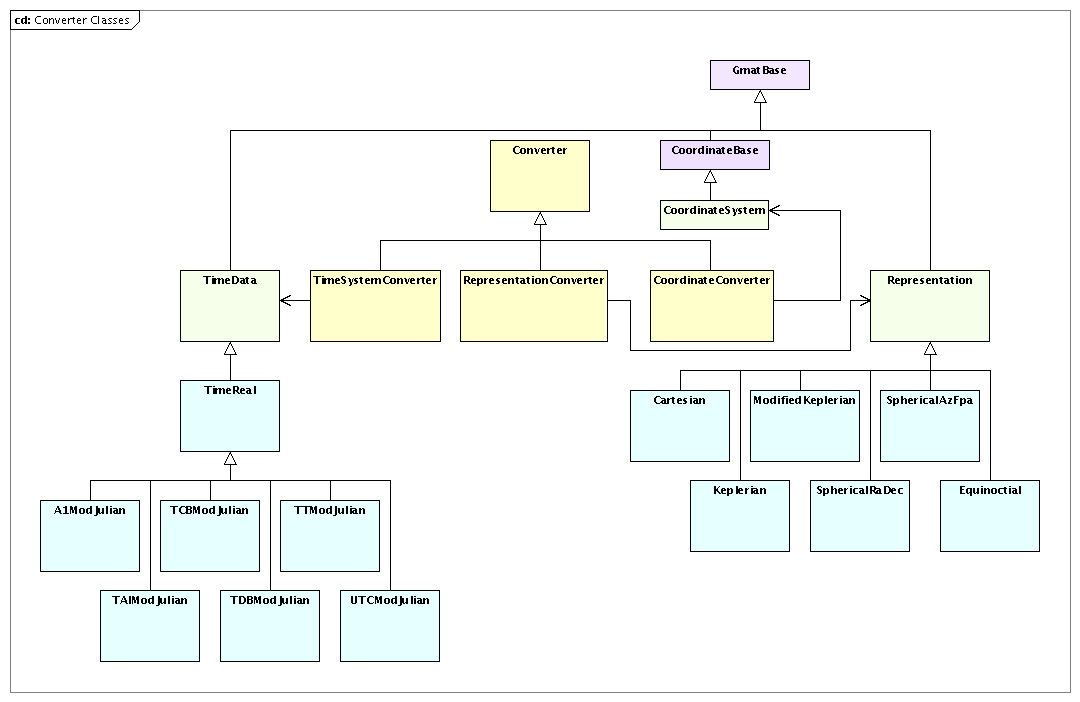
\includegraphics[scale=0.4]{Images/ConverterClasses.eps}
\caption[Classes Used to Provide Views of the SpaceObject State
Data]{\label{figure:SpaceObjectMVCClasses}Classes Used to Provide Views of the SpaceObject
State Data.  The converter classes are shown in yellow.  Base classes for the View support classes
are green, and specific support classes are shown in blue.}
\end{center}
\end{figure}

The class hierarchy for the converters and the support classes is shown in
Figure~\ref{figure:SpaceObjectMVCClasses}\footnote{Figure~\ref{figure:SpaceObjectMVCClasses} shows
the long term design for the conversion classes.  The code base developed for the first release of
GMAT supports the interfaces needed for conversion, but only partially implements the illustrated
design.}.  Each converter is derived from the Converter base class.  All converters support the
ability to take a PropState and transform the data in that state into the requested format for
display and manipulation by the user.  They also support the inverse operation, converting a set of
user data specified into a PropState.  The interfaces for these conversions are contained in the
Converter base class.

Each Converter subclass holds a reference to the data type used in the PropState as the base
representation for the corresponding data.  The object that owns the PropState is responsible for
setting this reference.

\subsection{The Converter Base Class}

All conversions performed for spacecraft and formations are managed through the Converter classes.
GMAT provides three types of converters: time system converters, coordinate system converters, and
state representation converters.  Each of these converters manages the corresponding conversion
code.  The SpaceObjects wrap these calls in methods that simplify interface to the data.  Specific
conversions are made through the calls to the Convert method on the appropriate converters.

The Converter base class has the following internal data members and methods:

\subparagraph{\textit{Class Attributes}}

\begin{itemize}
\item \textbf{static StringArray supportedConversions}: String array of all of the defined
conversions supported by this converter.
\item \textbf{Integer precision}: Precision used for numeric data when converting to a string
format.
\end{itemize}

\subparagraph{\textit{Methods}}

\begin{itemize}
\item \textbf{void Initialize()}: Method called to prepare and validate the converter for use in a
SpaceObject.
\item \textbf{static bool AddConversion(const std::string \&conversionType, GmatBase *toBase)}:
Method used to add support for a new conversion to the Converter.  This method is used to add
configured CoordinateSystems to the CoordinateConverter.  The TimeConverter and
RepresentationConverter classes do not support addition of new systems in the current builds of
GMAT.
\item \textbf{static StringArray GetSupportedConversions()}: Method used to return the list of all
of the conversions supported by the Converter.
\item \textbf{std::vector<Real> Convert(const PropState \&fromState, std::string toType,
GmatBase*=NULL
toObject) = 0}: Abstract method that converts data from a PropState into the requested type.
\item \textbf{PropState Convert(std::vector<Real> fromState, std::string fromType, GmatBase*=NULL
fromObject) = 0}: Abstract method that fills a PropState in the internal representation from
input data of the specified type.
\item \textbf{virtual StringArray ToString(std::string toFormat, std::vector<Real> value,
std::string fromFormat) = 0}: Abstract conversion routine that takes a state in Real vector
(\texttt{value}) in a specified format (\texttt{fromFormat}) and converts it to a string array in a
target format (\texttt{toFormat}).
\item \textbf{virtual std::vector<Real> ToReal(std::string fromFormat, StringArray value,
std::string toFormat) = 0}: Abstract conversion routine that takes a the text form of a state in
StringArray (\texttt{value}) in a specified format (\texttt{fromFormat}) and converts it to a Real
vector in a target format (\texttt{toFormat}).
\end{itemize}

\subsection{Time Conversions}

The TimeConverter class provides implementations for the abstract methods inherited from the
Converter base class.  The current code base supports time conversions using C-style functions
enclosed in a namespace, TimeConverterUtil.  The TimeConverter class wraps these conversions so
that there is a time conversion interface in GMAT that looks identical to the other conversion
interfaces in the system.  A future release of the system will rework the time conversions do that
the class structure matches the class hierarchy shown in Figure~\ref{figure:SpaceObjectMVCClasses}.
 The following descriptions provide initial steps toward this goal, marked as with the prefix
``<<Future>>'' for elements that are not planned for the system until these elements are
incorporated during these time system revisions\footnote{GMAT is, by design, extensible to
incorporate new components as they are identified and constructed by the GMAT community, without
violating the integrity of the official code base. The time system code as currently implemented
would require rework in the GMAT's base code to support any new time system, violating this
requirement; the design shown here provides the framework needed to correct this discrepancy.}.

\begin{figure}[htb]
\begin{center}
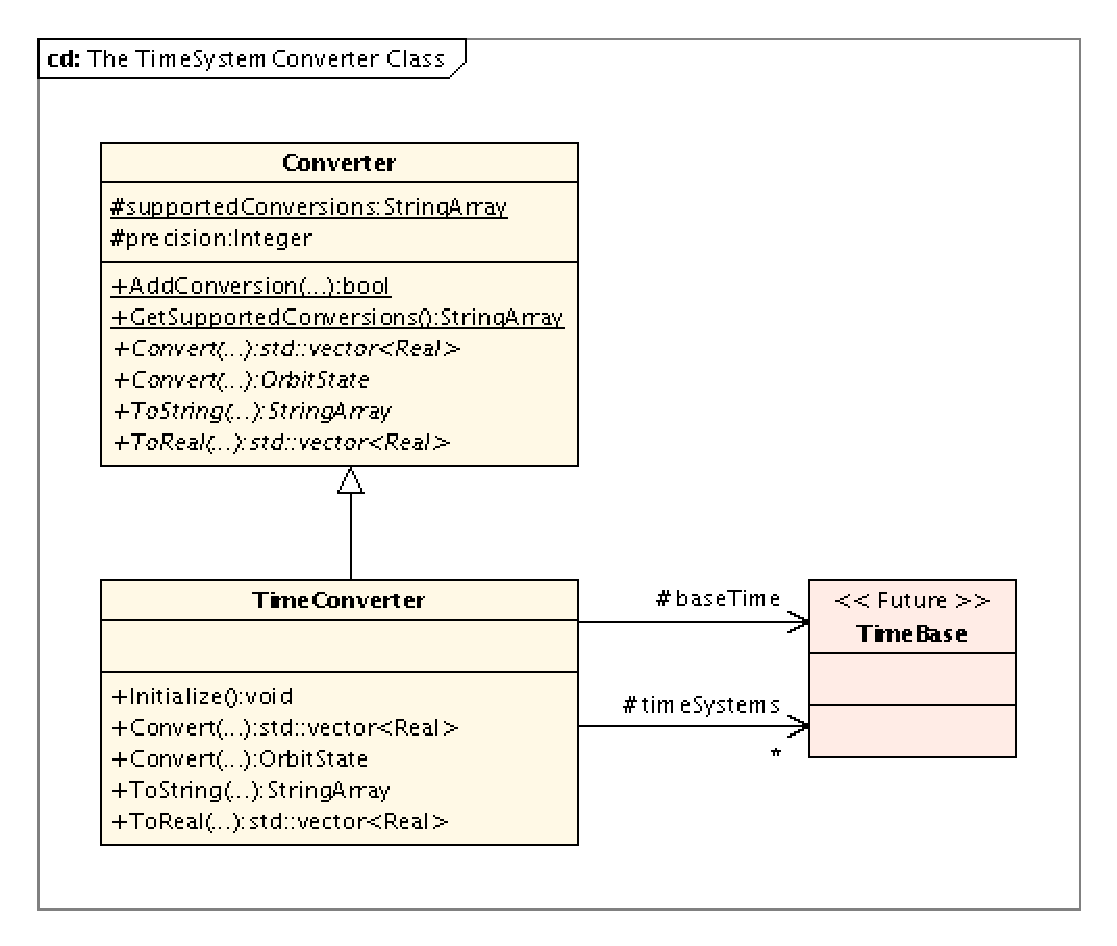
\includegraphics[scale=0.5]{Images/TheTimeSystemConverterClass.eps}
\caption{\label{figure:TimeConverterClasses}Classes Used to Convert Epoch Data}
\end{center}
\end{figure}

The TimeConverter class is shown in Figure~\ref{figure:TimeConverterClasses}.  The properties of
this class, including the arguments for the methods that are hidden in the figure, are tabulated
below.

\subparagraph{\textit{Class Attributes}}

\begin{itemize}
\item \textbf{<<Future>> TimeBase *baseTime}: An instance of the base time system used internally in
GMAT. This member contains a pointer to a TAIModJulian instance so that the conversion code has the
time system for methods that use PropStates at one end of the conversion.
\item \textbf{<<Future>> std::vector<TimeBase*> timeSystems}: A vector containing pointers to
each of the defined time systems in GMAT, so that the conversion code can perform conversions
without requiring time system pointers on the function calls.
\end{itemize}

\subparagraph{\textit{Methods}}

\begin{itemize}
\item \textbf{void Initialize()}: Method called to prepare and validate the converter for use in a
SpaceObject.
\item \textbf{std::vector<Real> Convert(const PropState \&fromState, std::string toType,
GmatBase*=NULL
toObject)}: Method that converts the TAI epoch data from a PropState into the requested type.
The resulting modified Julian data is stored in the first element of the returned array.
\item \textbf{PropState Convert(std::vector<Real> fromState, std::string fromType, GmatBase*=NULL
fromObject)}: Method that sets the epoch on a PropState to the epoch contained as the first
element in the input data (\texttt{fromState}), which is expressed in the time system given by the
name in the \texttt{fromType} string.
\item \textbf{virtual StringArray ToString(std::string toFormat, std::vector<Real> value,
std::string fromFormat) = 0}: Conversion routine that takes epoch data in a vector of Reals in a
specified format (\texttt{fromFormat}) and produces the string equivalent of each element in the
requested format, given by \texttt{toFormat}, in the returned StringArray.
\item \textbf{virtual std::vector<Real> ToReal(std::string fromFormat, StringArray value,
std::string toFormat) = 0}: Conversion routine that takes one or more epochs in a StringArray
(\texttt{value}) in a specified format (\texttt{fromFormat}) and converts them into a vector of
Real data in a target format (\texttt{toFormat}).  The resulting data is a vector of modified
Julian data in the target time system.  If a request is made from Gregorian data in the Real
vector, an exception is thrown.
\end{itemize}

\subsubsection{The TimeSystem Classes}

As mentioned above, the current time system conversion code does not use a class bases system to
handle the time systems.  This section will be completed when the time system code is brought into
conformance with the conversion system design.

\subsection{Coordinate System Conversions}

Figure~\ref{figure:CoordinateConverterClasses} shows the CoordinateConverter class, used to
transform state data between different coordinate systems.  The CoordinateConverter class works
with state data expressed in Cartesian coordinates exclusively.  Consumers that have state data in
other representations first convert the data into Cartesian coordinates, and then use the
facilities provided by instances of this class to transform between coordinate systems.

\begin{figure}[htb]
\begin{center}
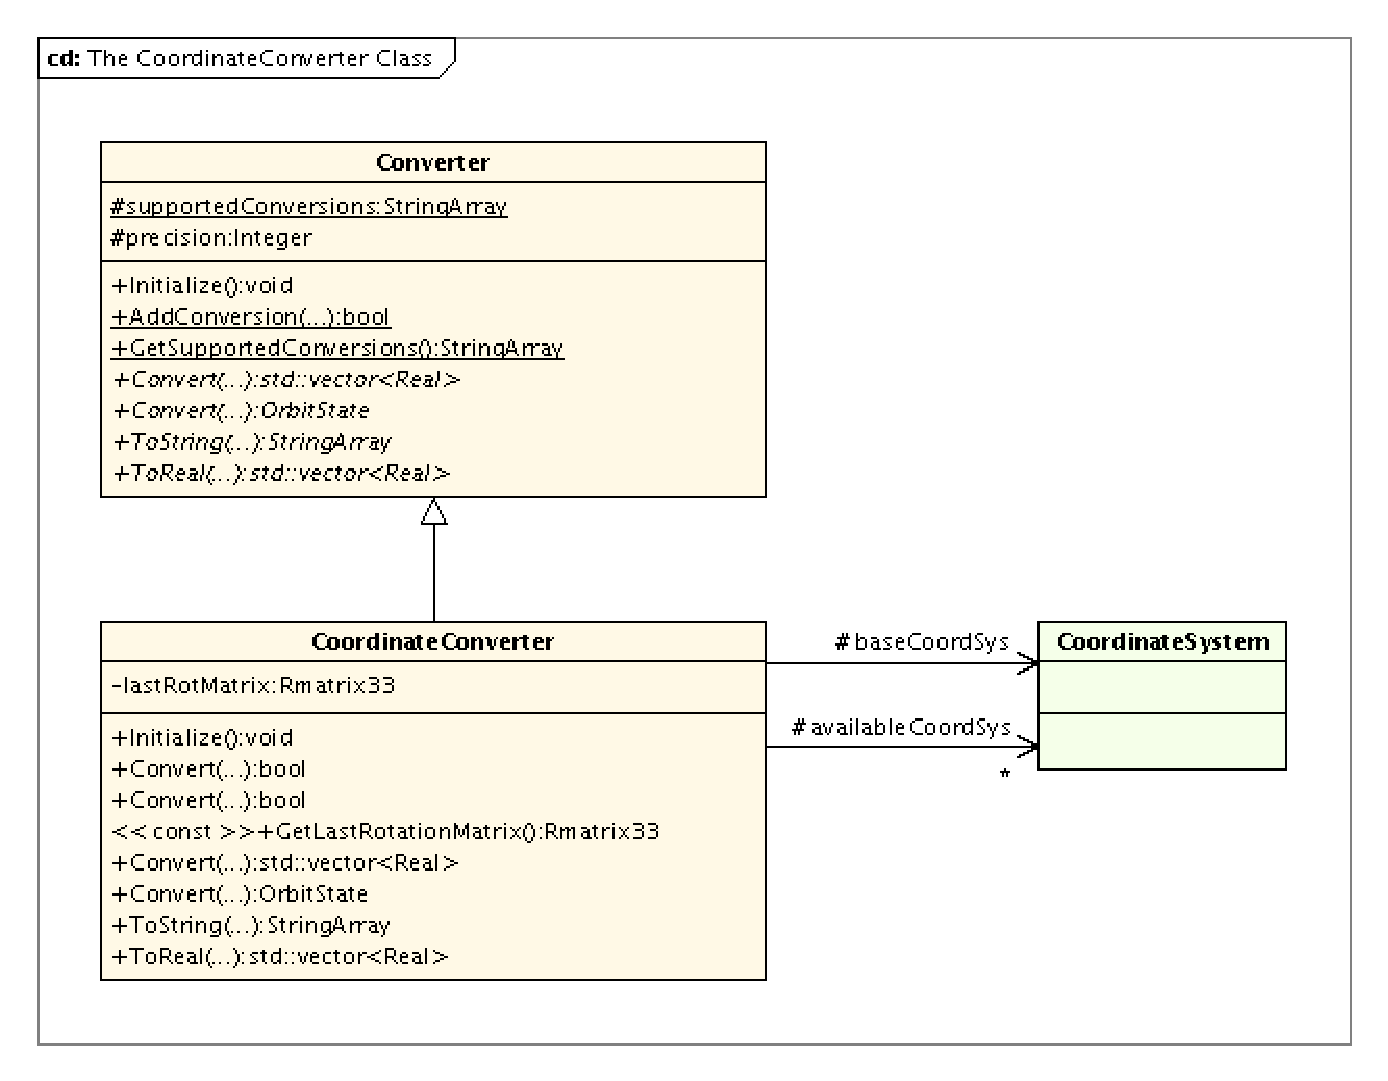
\includegraphics[scale=0.5]{Images/TheCoordinateConverterClass.eps}
\caption{\label{figure:CoordinateConverterClasses}Classes Used to Convert Between Coordinate
Systems}
\end{center}
\end{figure}

The CoordinateConverter objects work with any coordinate system defined by the user.  The other two
converters provided by GMAT -- the TimeConverter class and the RepresentationConverter class --
require code compiled into GMAT in order to function\footnote{A future release of GMAT may allow
dynamic definition of representations and time systems.  That facility is not planned for near term
GMAT functionality.}.  Coordinate systems in GMAT can be defined at run time, as described in
\cite{userGuide}.  The dynamic nature of these objects requires greater versatility in the
conversion
methods.  Consumers of these methods must provide pointers to instances of the coordinate systems
used in the conversions.

\subsubsection{CoordinateConverter Attributes and Methods}

\subparagraph{\textit{Class Attributes}}

\begin{itemize}
\item \textbf{CoordinateSystem *baseCoordSys}: An instance of the CoordinateSystem class used as
the base class for conversions involving a PropState.  This member is initialized to NULL, and set
by SpaceObjects that need it prior to use.
\item \textbf{Rmatrix33 lastRotMatrix}: The most recent rotation matrix used in coordinate
conversions, stored so that it can be accessed externally.
\item \textbf{std::map <std::string, CoordinateSystem*> availableCoordSys}: A map of coordinate
systems available for use in methods that do not pass on CoordinateSystem pointers.  These pointers
are stored in a map so that they can be accessed by name.
\end{itemize}

\subparagraph{\textit{Methods}}

\begin{itemize}
\item \textbf{void Initialize()}: Method called to prepare and validate the converter for use in a
SpaceObject.
\item \textbf{bool Convert(A1Mjd epoch, Rvector inState, CoordinateSystem* inCoord, Rvector
outState, CoordinateSystem* outCoord, bool forceNutationComputation = false, bool omitTranslation =
false)}: General purpose conversion routine that converts a Cartesian Rvector in a given input
coordinate system into a Cartesian Rvector in the output coordinate system.
\item \textbf{bool Convert(A1Mjd epoch, Real* inState, CoordinateSystem* inCoord, Real* outState,
CoordinateSystem* outCoord, bool forceNutationComputation=false, bool omitTranslation=false)}:
General purpose conversion routine that converts a Cartesian Real array in a given input
coordinate system into a Cartesian Real array in the output coordinate system.  This method
requires that the input and output Real arrays both contain the Cartesian state in the first six
elements.
\item \textbf{Rmatrix33 GetLastRotationMatrix() const}:  Method used to access the most recent
rotation matrix used in conversions.
\item \textbf{std::vector<Real> Convert(const PropState \&fromState, std::string toType, GmatBase*
toCS)}: Method that converts the state in the input PropState into the specified CoordinateSystem.
The toCS parameter is a pointer to an instance of the target coordinate system.  This method
uses the base coordinate system, baseCoordSys, as the coordinate system of the input PropState.
The calling code must ensure that the base coordinate system is set correctly.
\item \textbf{PropState Convert(std::vector<Real> fromState, std::string fromType, GmatBase*
fromCS)}: Method that sets the state in the data in a PropState in the base coordinate system,
given an input state in a specified CoordinateSystem.  The \texttt{fromCS} parameter is a pointer to
an instance of the coordinate system used for the input state, \texttt{fromState}.  This method
uses the base coordinate system, baseCoordSys, as the coordinate system of the target PropState.
The calling code must ensure that the base coordinate system is set correctly.
\item \textbf{StringArray ToString(std::string toFormat, std::vector<Real> value, std::string
fromFormat)}:  Method that takes a Cartesian state contained in a vector of Reals is a specified
coordinate system, and converts it into a target coordinate system, then stores the data in a
StringArray at the precision set for the converter.
\item \textbf{std::vector<Real> ToReal(std::string fromFormat, StringArray value, std::string
toFormat)}: Method that takes a Cartesian state contained in a StringArray in a specified
coordinate system, and converts it into a target coordinate system, then stores the data in a
vector of Reals.
\item \textbf{void AddCoordinateSystem(CoordinateSystem *cs)}: Method used to add a CoordinateSystem
pointer to the map of available coordinate systems.
\end{itemize}

\subsubsection{The CoordinateSystem Classes}

Coordinate Systems in GMAT are described in detail in Chapter~\ref{chapter:CoordinateSystems}.

\subsection{State Representation Conversions}

Once the coordinate system has been selected for a state, the actual format for the data must also
be selected.  The state can be displayed in many different ways: as Cartesian data, as the
corresponding Keplerian elements, or in any other representation defined in GMAT.  The conversion
from the Cartesian state into a selected representation is managed by the RepresentationConverter
class, shown in Figure~\ref{figure:RepresentationConverterClasses}.

\begin{figure}[htb]
\begin{center}
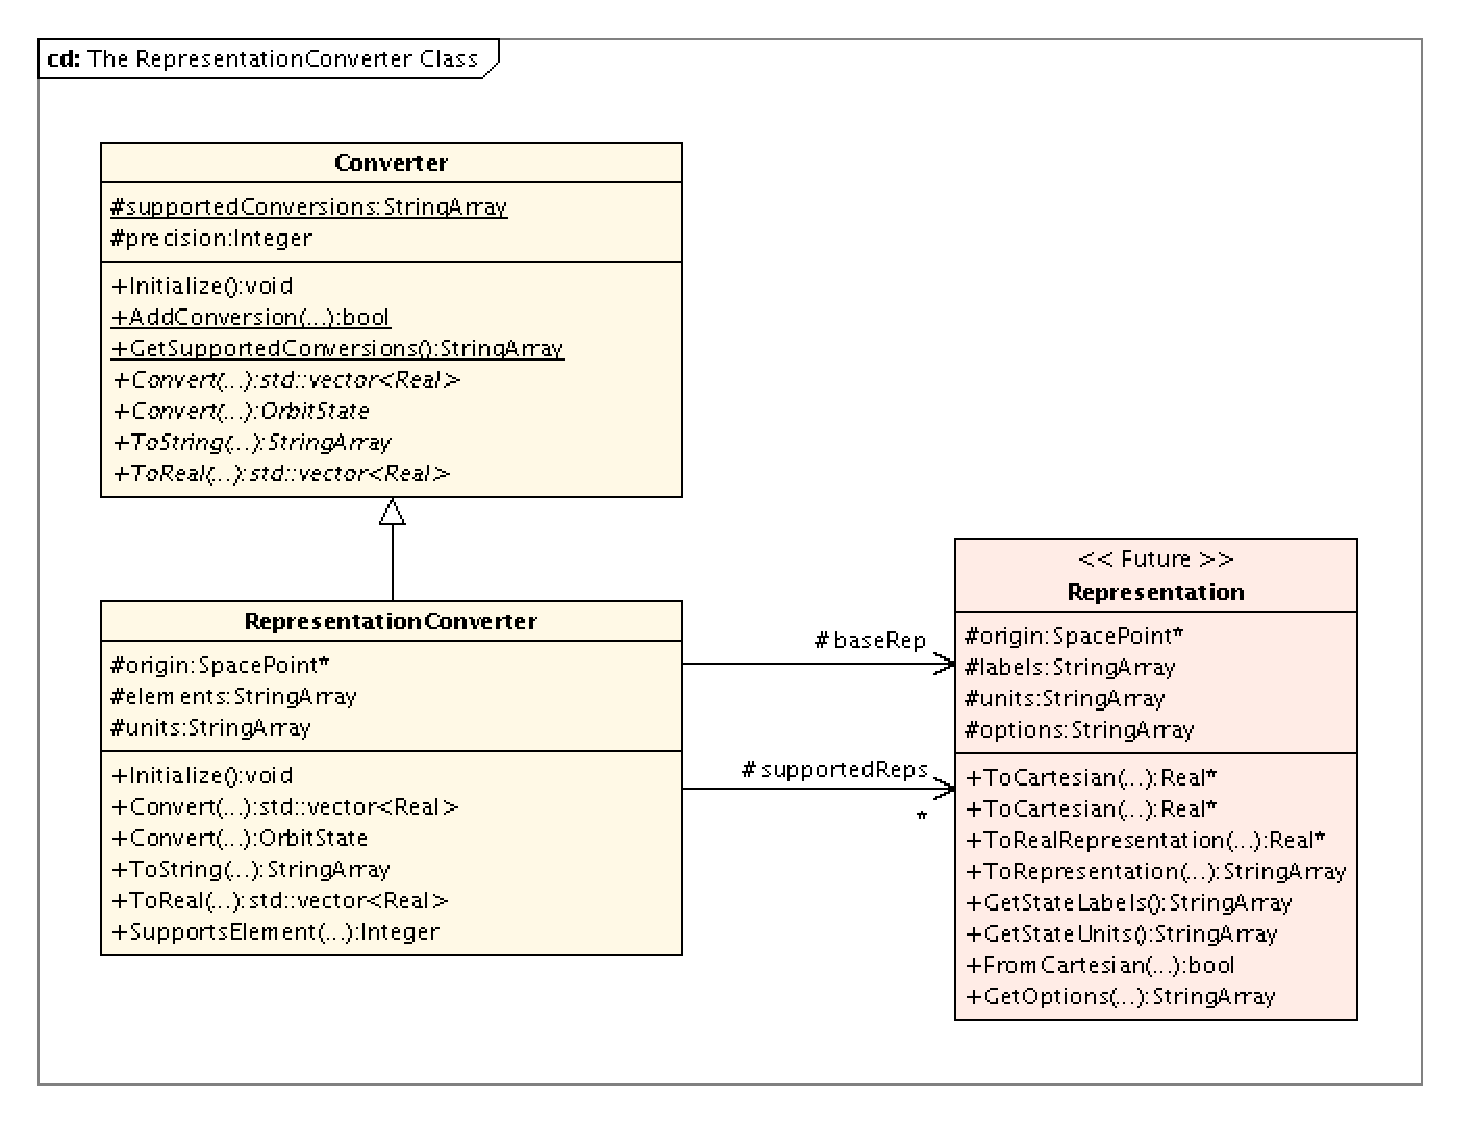
\includegraphics[scale=0.5]{Images/TheRepresentationConverterClass.eps}
\caption{\label{figure:RepresentationConverterClasses}Classes Used to Convert State Representations}
\end{center}
\end{figure}

\subsubsection{RepresentationConverter Attributes and Methods}

\subparagraph{\textit{Class Attributes}}

\begin{itemize}
\item \textbf{SpacePoint* origin}: The SpacePoint defining the coordinate system origin.  Some
representations need this object to determine the representation data; for instance, the Keplerian
representation needs the gravitational constant for the body at the origin.
\item \textbf{StringArray elements}: A vector of text string labels for the elements.  This
vector contains the labels for the most recent target conversion.
\item \textbf{StringArray units}: A vector of text string labels for the element units.  This
vector contains the units for the most recent target conversion.
\item \textbf{<<Future>> Representation baseRep}: The representation used for the PropState data.
\item \textbf{<<Future>> std::vector<Representation*> supportedReps}: A vector of instances of all
supported representations, provided so that conversions can be made without passing in a pointer to
a target representation.
\end{itemize}

\subparagraph{\textit{Methods}}

\begin{itemize}
\item \textbf{<<Future>> bool AddRepresentation(Representation* rep)}: Method used to register a new
representation with the converter.  This method is used to register new representations that are
built into shared libraries loaded at run time.
\item \textbf{std::vector<Real> Convert(const PropState \&fromState, std::string toType, GmatBase*
toRep=NULL)}: Method that converts the state in the input PropState into the specified
Representation.  The optional toRep parameter is a pointer to an instance of the target
Representation; if it is not provided, the converter finds an instance in its internal array of
Representations.  This method uses the base representation, baseRep, as the representation of the
input PropState.  The calling code must ensure that the base representation is set correctly.
\item \textbf{PropState Convert(std::vector<Real> fromState, std::string fromType, GmatBase*
fromRep)}: Method that sets the state in the data in an PropState in the base representation,
given an input state in a specified Representation.  The \texttt{fromRep} parameter is a pointer to
an instance of the Representation used for the input state, \texttt{fromState}.  This method
uses the base Representation, baseRep, as the representation of the target PropState.  The calling
code must ensure that the base representation is set correctly.
\item \textbf{std::string SupportsElement(std::string label)}: Method used to query all supported
representations to determine which representation supports a specified element.  The return value
is the name of the supporting representation.
\item \textbf{StringArray ToString(std::string toFormat, std::vector<Real> value,
std::string fromFormat="Cartesian")}: Conversion routine that generates a text view of the state
contained in the input Real vector in a target representation.  The resulting StringArray contains
data at the Converter's precision.
\item \textbf{std::vector<Real> ToReal(std::string fromFormat, StringArray value,
std::string toFormat="Cartesian")}: Conversion routine that takes a text version of a state in
a StringArray, expressed in a specified representation, and converts it into a Real vector of data
in a target representation.
\end{itemize}

\subsubsection{The Representation Classes}

<<Future>>\footnote{Like the time conversion classes, the representation conversion classes
do not currently conform to the design presented here.  Accordingly, in the following descriptions,
the elements that are not planned for immediate implementation are marked as future enhancements.}
All state representations share a common interface, enforced by the Representation base class.
Representations like the Keplerian representation that provide options for certain elements provide
the list of options for the elements on an element by element basis..

\section{\label{section:SpaceObjectConversions}Conversions in SpaceObjects}

The SpaceObject classes -- SpaceObject, Spacecraft, and Formation, and other classes as they are
added to GMAT -- all share a common representation of locations in the GMAT SolarSystem, the
PropState.  As its name implies, the PropState class is the core component that interacts with the
propagation subsystem; it contains the epoch, position and velocity data that is advanced to model
the motion of user defined objects in the solar system.  The data stored in the PropState is a TAI
epoch and the Mean-of-J2000 Cartesian positions and velocities of the objects that are propagated.
The origin for these data is a SpacePoint object defined in the solar system.  Each SpaceObject
includes a pointer to the SPacePoint defining the origin and a CoordinateSystem object configured as
a Mean-of-J2000 Earth-Equatorial origin-centered coordinate system to facilitate conversions
between the data in the encapsulated PropState and external consumers of the data.

The PropState data is encapsulated inside of SpaceObject instances.  Users interact with the
PropState indirectly, by making calls to these SpaceObjects.  This feature provides a buffering
mechanism to GMAT's SpaceObjects, so that the data in the PropState can be formatted for
presentation purposes for the user.  The SpaceObject class provides interfaces that convert the
internal PropState data into other formats for display, and that take data from those formats and
convert them into the internal PropState structures needed for computation.

SpaceObjects include four data structures used this buffering of the state data.  The epochType and
stateType data members are strings containing the current settings for the displayed format of the
epoch and state representation.  String versions of the epoch and state in these formats are stored
in the textEpoch and textState data members.  These string versions of the data are the versions
that users interact with when configuring a mission, either from the GUI or using the scripting
interface.  The following paragraphs describe the procedure followed when performing these
interactions.

\subsection{SpaceObject Conversion Flow for Epoch Data}

\begin{figure}
\begin{center}
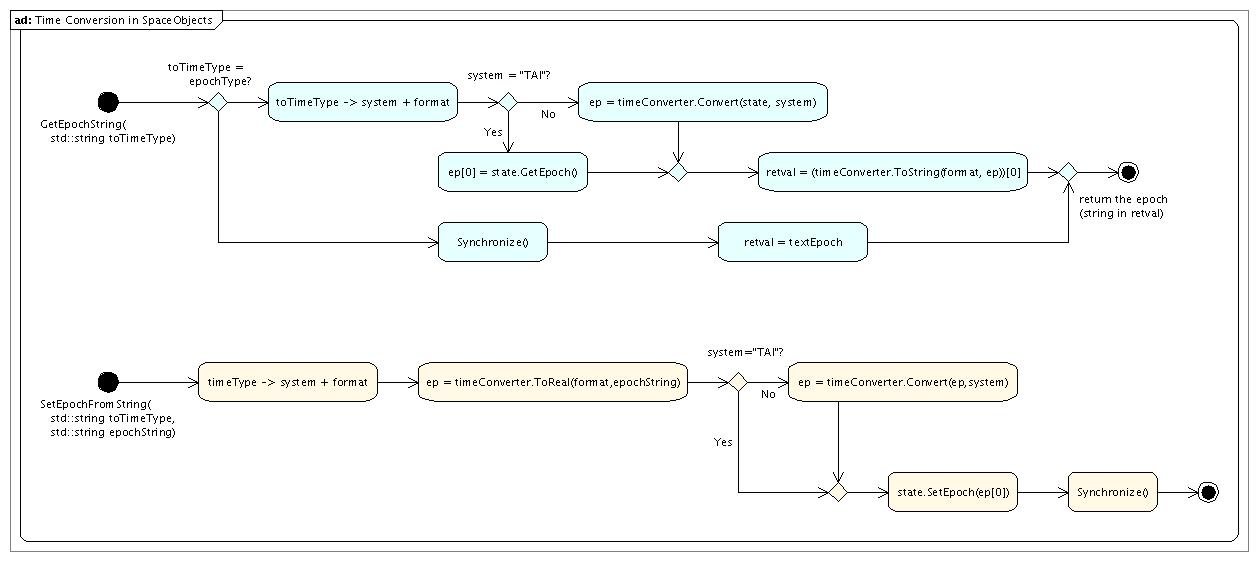
\includegraphics[scale=0.35]{Images/TimeConversioninSpaceObjects.eps}
\caption{\label{figure:TimeConversion}Procedure for Retrieving or Setting a Formatted Epoch}
\end{center}
\end{figure}

Figure~\ref{figure:TimeConversion} shows the procedure employed to send and receive epoch data for a
SpaceObject using the string format needed for display and output purposes.  Epochs can be
displayed in either Gregorian or Modified Julian format, using one of several different supported
time systems.  The time system used and the format for the output are separate entities, and
treated as such in GMAT.  The internal epoch data is stored in the TAI system as a Modified Julian
Real number.  This data is retrieved for external manipulation as a string, using the
GetEpochString() method on the SpaceObject that owns the epoch.  Updated epoch data is passed into
the SpaceObject using the SetEpochFromString method.

The top activity diagram in the figure shows the procedure followed to retrieve the current epoch
data from the SpaceObject using the GetEpochString method.  The first action taken is a test to
determine if the target time format matches the epoch format used in the SpaceObject.  If so, then
the string that is returned is the textEpoch data member for the SpaceObject, as set immediately
after synchronizing the textEpoch with the PropState.  If the time systems do not match, the target
time system is broken into two pieces: the time system used and the format for the string. The
format portion is the suffix on the toTimeType parameter, and is either ``ModJulian'' or
``Gregorian''.  The GetEpochString method retrieves the epoch from the PropState and, if the
 target system is not TAI, converts it into the target time system.  Then it takes that ModJulian
real number, and converts it into a formatted string using the timeConverter's ToString method.

The lower activity diagram in Figure~\ref{figure:TimeConversion} shows the procedure followed when
setting the epoch from the GUI or script, using the SetEpochString method on the SpaceObject.  The
first parameter in this call specifies the format of the input time.  It is broken into the input
time system and the format of the string.  The time converter then constructs a modified Julian
real value for the input string using its ToReal method.  If the input time is not a TAI time, it
is then converted into TAI.  The resulting modified Julian epoch is then set on the PropState using
the SetEpoch method.  Finally, the Synchronize method is called on the SpaceObject to update the
string representation of the epoch with the data in the PropState.

\subsection{SpaceObject Conversion Flow for State Data}

The state data in the PropState can be manipulated either element by element or as a complete
vector.  The following paragraphs describe the conversion procedures for both approaches.

\subsubsection{Converting State Vectors}

\begin{figure}[htb]
\begin{center}
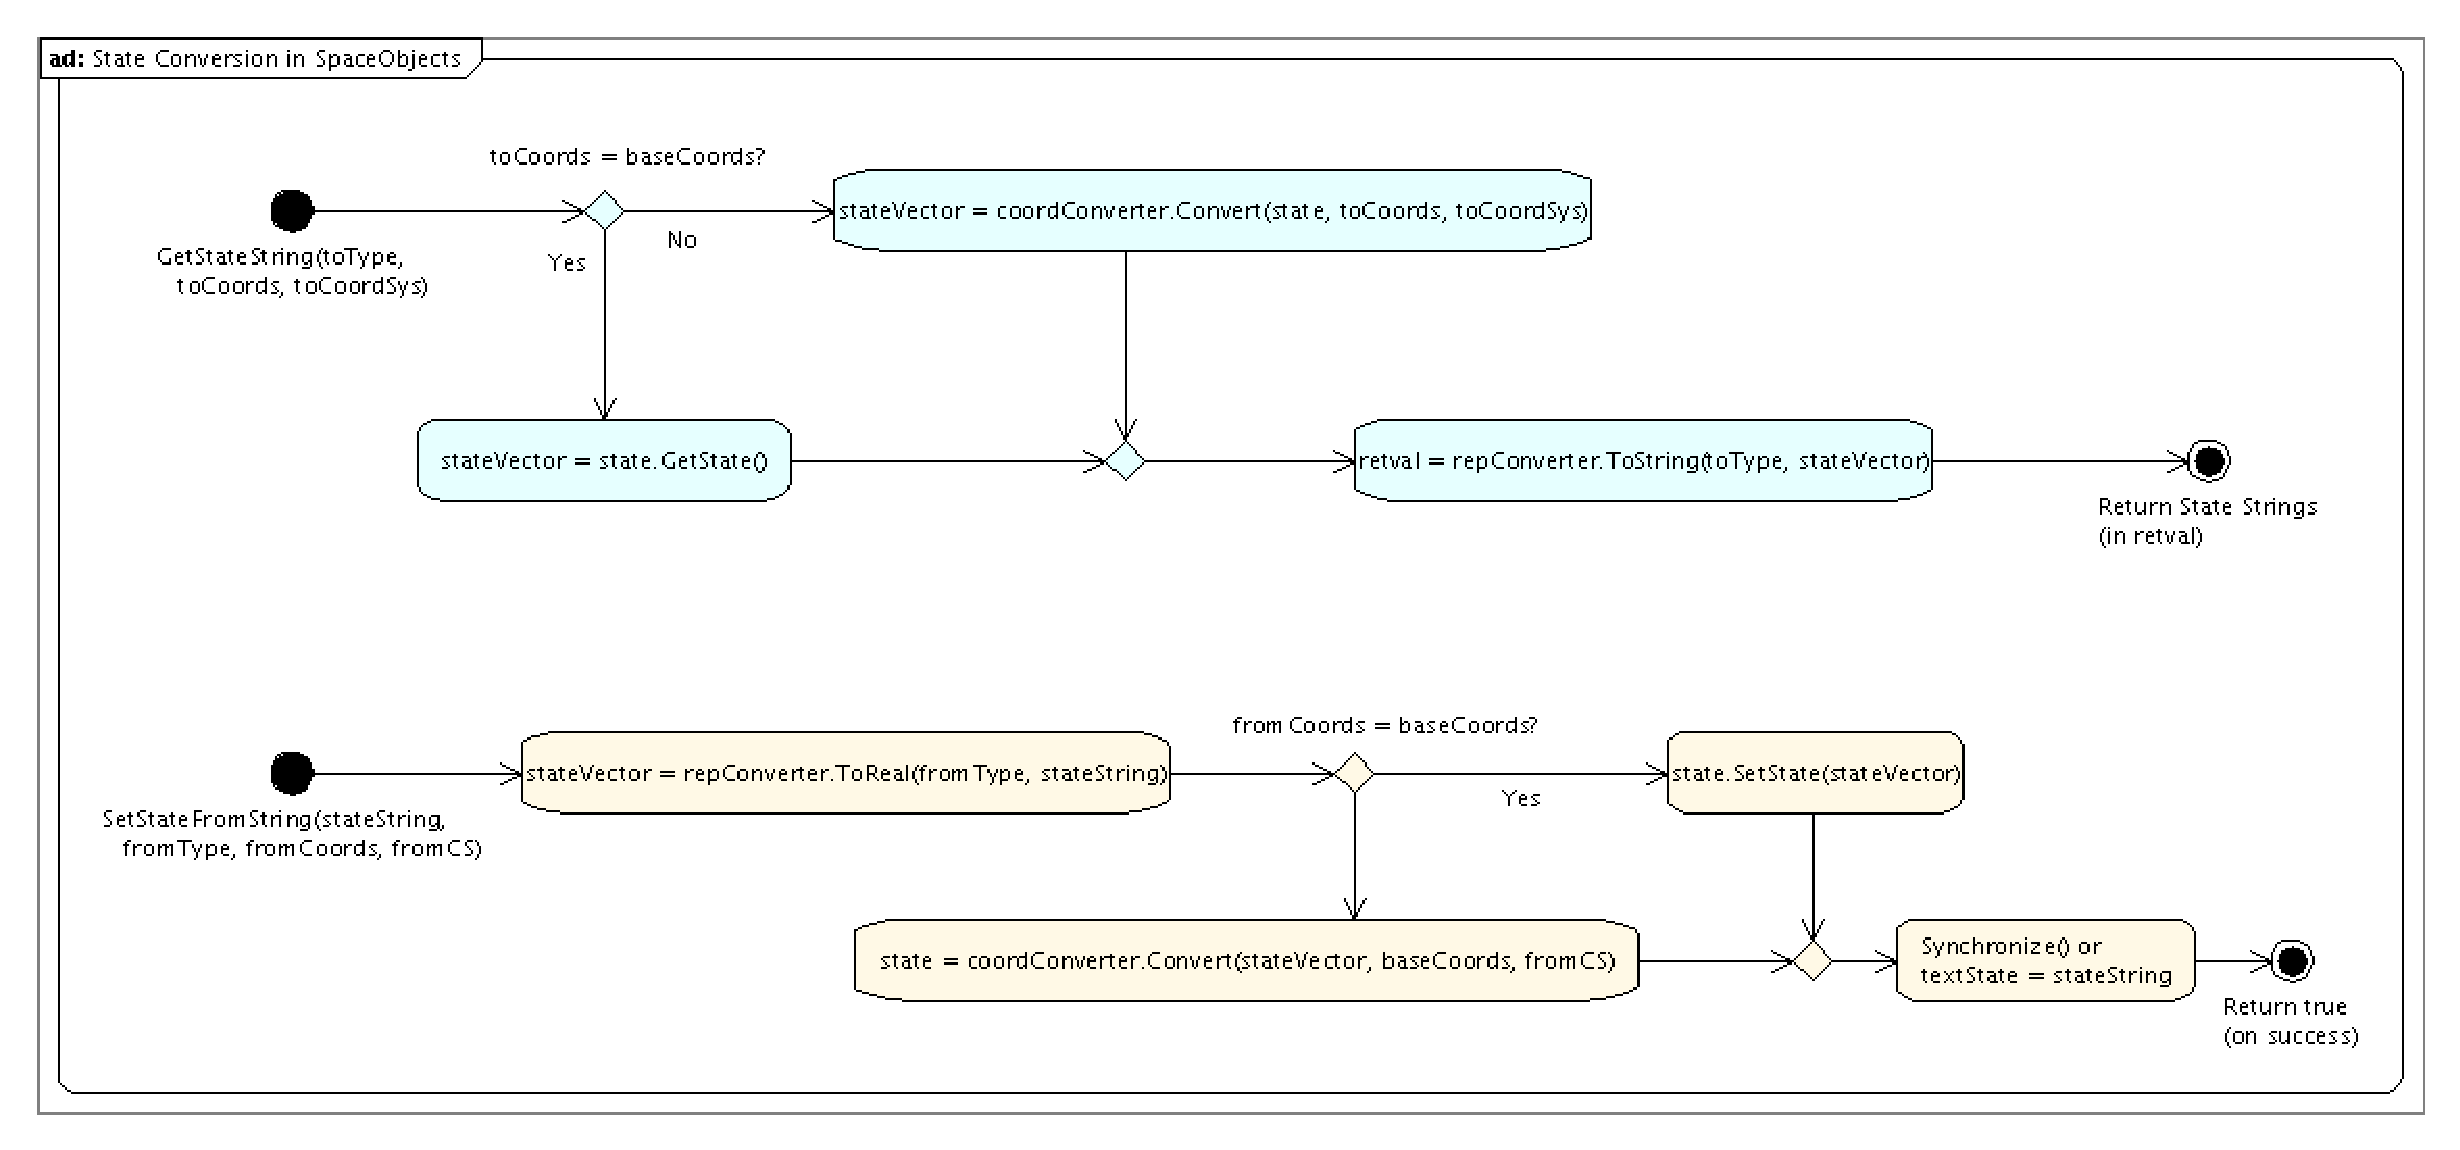
\includegraphics[scale=0.35]{Images/StateConversioninSpaceObjects.eps}
\caption{\label{figure:StateConversion}Procedure for Retrieving or Setting a Formatted State}
\end{center}
\end{figure}

Figure~\ref{figure:StateConversion} shows the procedures employed to convert the state in vector
form.  State conversions are always a two step procedure.  The state data in the PropState is
always defined with respect to the Mean-of-J2000 Earth Equatorial coordinate axes orientation, wit
h the coordinate origin located at a user specified origin. The internal data is stored in the
Cartesian representation\footnote{A future update will allow internal storage in either Cartesian
or Equinoctial elements, so that Variation of Parameters propagation methods can be implemented.}.
Users can view the state in any defined coordinate system using any representation defined in GMAT.
 Hence the procedure for building the state for display to the user potentially involves both a
coordinate transformation and an element conversion, as shown in the figure.

Conversion of the PropState data for display is shown in the top diagram in the figure.  The state
vector is requested using the GetStateString method, which contains three parameters: the target
representation in the toType parameter, the name of the target coordinate system in the toCoords
parameter, and a pointer to an instance of the target coordinate system.  The SpaceObject has a
pointer to a base coordinate system, along with the name of the base system.  If these match the
target coordinate system, then the coordinate conversion step can be skipped; otherwise, the
internal state vector in the PropState is converted into the target coordinate system.  The
resulting intermediate state vector is then converted into a StringArray in the target
representation using the ToString() method on the SpaceObject's representation converter.

The lower diagram in Figure~\ref{figure:StateConversion} shows the inverse process, used to set the
state vector on a SpaceObject through the SetStateFromString method.  This method has four
parameters: the input state in the StringArray parameter stateString, the representation that that
StringArray uses (fromType), the name of the coordinate system (fromCoords) used for the input
state, and a pointer to an instance of that coordinate system (fromCS).  First the input state is
converted into a Cartesian vector using the SpaceObject's RepresentationConverter.  Once the
Cartesian state has been constructed, it is transformed into the internal coordinate system and
stored in the SpaceObject's PropState.  Finally, the SpaceObject's text representation of the state
is updated suing the Synchronize method\footnote{If both the representation and internal coordinate
system for the PropState match the input values, the input state vector strings are copied into the
testState member, and Synchronize() is not called.}

\subsubsection{Converting Single Elements}

\begin{figure}[htb]
\begin{center}
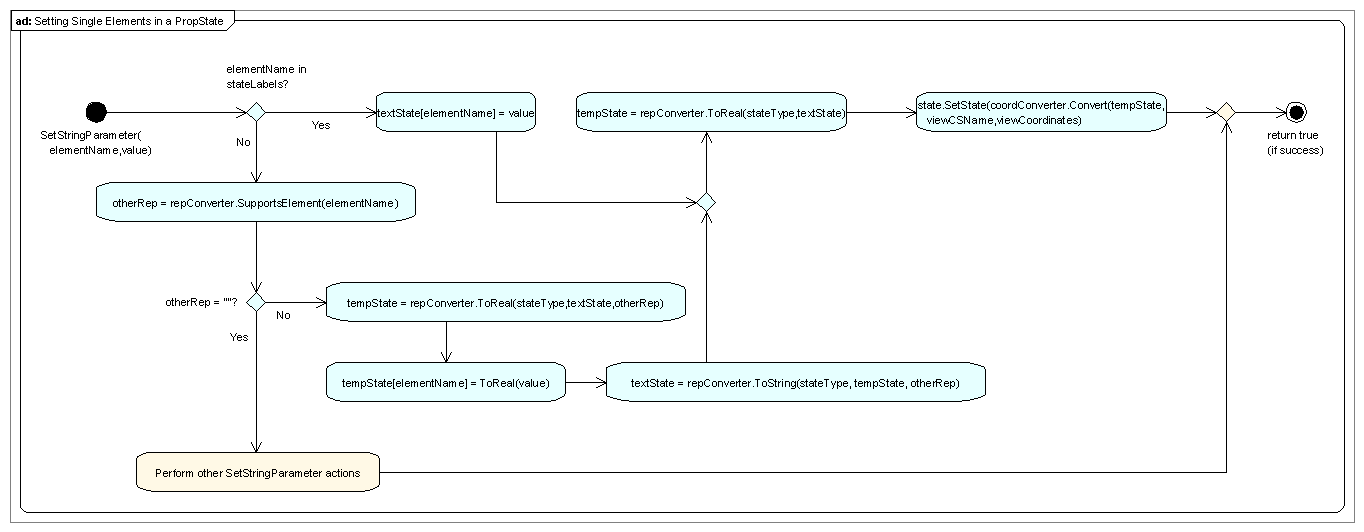
\includegraphics[scale=0.32]{Images/SettingSingleElementsinanOrbitState.eps}
\caption{\label{figure:StateElementConversion}Procedure for Setting a Single Element in the State}
\end{center}
\end{figure}

The procedure for setting single state elements is shown in
Figure~\ref{figure:StateElementConversion}.  This procedure is slightly more involved than the
procedure employed to set a complete state because the procedure includes provisions for setting
elements from one representation while maintaining a different text representation of the state in
the textState buffer.  This allows a user to script, for example, a semimajor axis for a spacecraft
that stores its state in a Cartesian representation.  Element setting is performed using the
standard SetStringParameter method defined for all GmatBase subclasses.

The procedure employed for setting a single element when the element's name is a member of the
current state representation is straightforward.  The string containing the new element data in
inserted into the textState string array, converted into a real vector in Cartesian coordinates by
the representation converter, and then into the internal coordinate system by the coordinate system
converter.  This state is set on the PropState.

If the element is not a member of the current representation, the procedure is slightly more
complicated. The textState is converted from the current state type into a vector of real numbers
in the representation containing the element that is being set.  The element is set to the input
value, and the resulting vector is converted back into the textState StringArray.  Then the
textState is converted into the internal representation and coordinate system as described in the
previous paragraph.
